\section{Context Window for Zero-Shot Prompting}\label{app:sampler}

\begin{algorithm}[tb]
\DontPrintSemicolon
\KwIn{seed row $s$, context length $L$, width bound $w$, and,
for each row $r$ in the database:
non-missing feature cells $\mathcal{C}(r)$,
P$\to$F neighbors $\mathcal{N}_{\text{P}\to\text{F}}(r)$,
F$\to$P neighbors $\mathcal{N}_{\text{F}\to\text{P}}(r)$ and
timestamp $\mathcal{T}(r)$
}
\KwOut{the set of database cells $C$ in the context window}
$C \gets \{\}$, $F \gets \{s\}$ \tcp*[r]{F is the frontier of rows to explore}
\While{$|C| < L \land F \not= \{\}$}{
\tcc*[c]{select a row to explore; R is the set of candidates}
$R \gets \{r \in F \mid r$ was added via an F$\to$P link$\}$
\tcp*[r]{F$\to$P linked rows}
\If{$R = \{\}$}{
$R \gets \arg\min_{r \in F} \textsc{HopDistance}(r, s)$ \tcp*[r]{rows closest to $s$}
}
$r \gets \textsc{RandomSelect}(R)$ \tcp*[r]{pick a row at random}
$F \gets F \setminus \{r\}$ \tcp*[r]{remove row from frontier}
\leIf{$r$ has been visited}{
	continue
}{
	mark $r$ as visited
}
\tcc*[c]{visit row}
$C \gets C \cup \mathcal{C}(r)$
\tcp*[r]{add cells to context}
$F \gets F \cup \mathcal{N}_{\text{F}\to\text{P}}(r)$
\tcp*[r]{add F$\to$P neighbors to frontier}
$N \gets \{q \in \mathcal{N}_{\text{P}\to\text{F}}(r) \mid
\mathcal{T}(q) \le \mathcal{T}(s)\}$
\tcp*[r]{filter P$\to$F neighbors by time}
$N \gets \textsc{RandomSample}(N, w)$ \tcp*[r]{pick $\le w$ P$\to$F neighbors at random}
$F \gets F \cup N$ \tcp*[r]{add P$\to$F neighbors to frontier}
}
\KwRet{$C$}\;
\caption{
Sampling the context window of Relational Transformer.
We use a modified Breadth-First Search (BFS) algorithm,
with accommodations for relational-specific considerations,
such as F$\to$P links and temporal constraints. %\ck{I suggest this goes to the appendix}
}
\label{alg:sampler}
\end{algorithm}

\begin{figure}[t]
    \centering
    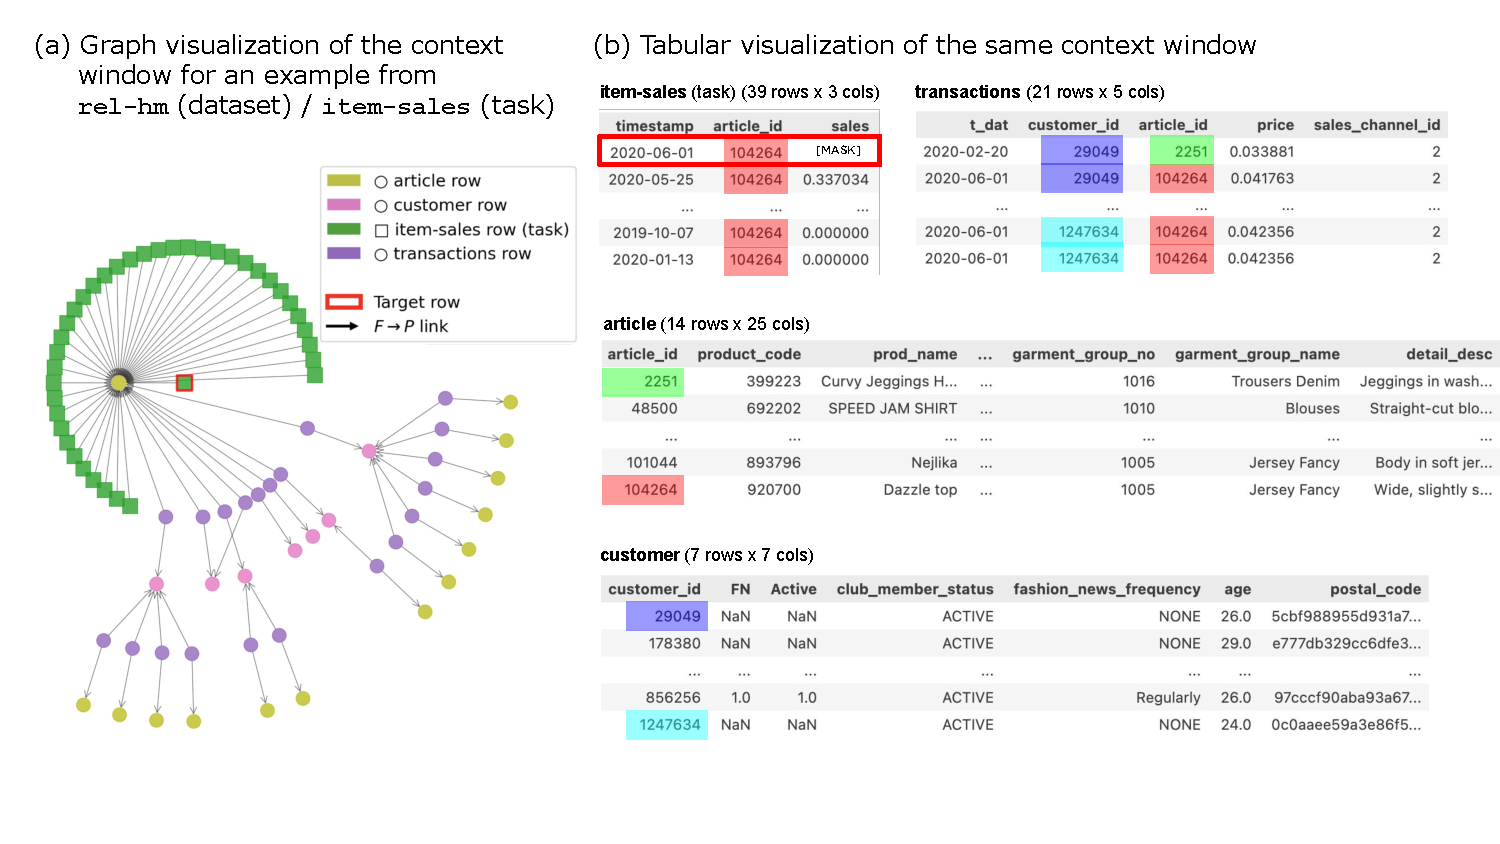
\includegraphics[width=\linewidth,trim={5 40 0 0},clip]{manual-figures/sampler-viz.pdf}
    \captionof{figure}{
Visualization of a real context window used for zero-shot prompting,
sampled by Alg.~\ref{alg:sampler} with
context length $L = 512$ and BFS width bound $w = 128$.}
    \label{fig:sampler-viz}
\end{figure}


\paragraph{Sampling cells for the context window.}
In \S~\ref{sec:background}, prediction tasks such as forecasting and autocompletion are framed as predicting a masked cell in the appropriate row (the \emph{seed row}). We sample the context window independently for each training/testing example, so there is always a unique seed row for context construction. Given the seed row and context length $L$, a suitable algorithm should select the cells most relevant to predicting the masked cell. Since relevance requires strong models to estimate accurately, we use a simple heuristic guided by the intuition that most relevant information lies within a few hops of the seed row when following F$\to$P and P$\to$F links, and that lower hops are more informative than higher hops.

We treat rows as the sampling unit: once a row is selected, all its non-missing feature cells (i.e., cells not from primary- or foreign-key columns) are included in the context. After the seed row, other rows are added using a bounded-width BFS across F$\to$P and P$\to$F links, with the following modifications: (1) F$\to$P links are immediately followed; (2) the traversal stops when the total number of cells reaches the context length; (3) unvisited rows at the same depth from the seed row are sampled uniformly; and (4) rows with timestamps greater than the seed row's timestamp are skipped (temporal constraint). The algorithm is summarized in Alg.~\ref{alg:sampler}. We use a fast, optimized Rust implementation to prevent on-the-fly sampling from slowing down training. Fig.~\ref{fig:sampler-viz} shows an example of sampled context window.

In Alg.~\ref{alg:sampler}, F$\to$P and P$\to$F links are treated asymmetrically. The number of F$\to$P links from a row is limited by the number of foreign-key columns in that table, and each parent row typically contains important features (e.g., a \texttt{transaction} row links to \texttt{user} and \texttt{product}). Conversely, P$\to$F links can have unbounded degree; informative signals from P$\to$F links often arise via aggregation, with diminishing returns from including many children. Thus we prioritize F$\to$P links (followed immediately without subsampling) and subsample P$\to$F links by enforcing a width bound $w$ (i.e., follow at most $w$ children from any row).



\section{Expanded Related Work}
\label{appsec:related_work}

\paragraph{Relational deep learning (RDL).} \citet{rdl} introduced an end-to-end framework for predictive modeling on relational databases using neural networks. At its core, RDL represents a database as a relational entity graph: a temporal, heterogeneous graph where each table is a node-type, each row an individual node, and every primary-foreign key relationship an edge. Initial approaches applied heterogeneous graph neural networks directly to these relational entity graphs~\citep{relbench}, and more recently, advanced message-passing approaches have been proposed to enhance the efficiency of GNNs on relational data~\citep{relgnn}. Transformers have emerged as a way to improve upon the GNN message-passing paradigm. \citet{dbformer} and \citet{relgt} propose transformer-based architectures that achieve better performance than GNNs on relational data. An review of RDL architecture can be found in \cite{dwivedi2025relational}. A key limitation, however, is that these architectures are schema-specific, which prevents pretraining and fine-tuning on diverse database structures. Our Relational Transformer, by design, is schema-agnostic, enabling it to learn from and be directly applied to new, unseen database structures. This design principle allows our architecture to demonstrate foundation model-like capabilities, similar to those recently shown in tabular learning.

\paragraph{Tabular foundation models (TFMs).}
Recent advancements in tabular foundation models have demonstrated significant promise, exhibiting capabilities such as in-context learning~\citep{tabpfn, tabicl} and efficient fine-tuning~\citep{carte}. 
These efforts have explored both supervised~\citep{tabpfn} and self-supervised~\citep{portal, carte}  pretraining on real~\citep{carte} or synthetic~\citep{tabpfn, tabicl} data.
Extending tabular foundation models to relational data is non-trivial, because not only are there multiple tables, but rows in one table are linked to rows in another by foreign-primary key links.
We take inspiration for the universal cell encoders/decoders from PORTAL~\citep{portal}, which has a similar handling of column names and text/numeric/datetime data types.
We also take inspiration from the TabPFNv2~\citep{tabpfnv2} transformer architecture, which uses stacked layers of row-wise and then column-wise attention, except that we also have all-pair attention and use attention masks to capture
foreign-primary key links.


\paragraph{Relational foundation models (RFMs).}
While tabular foundation models can, in principle, be applied to relational datasets, they fail to account for the rich, multi-table structure of real-world data. To address this limitation, recent works have begun to develop dedicated relational foundation models.
For instance, \citet{kumorfm} propose a relational foundation model based on graph-transformers and in-context learning, demonstrating both in-context learning and fine-tuning capabilities. However, their solution is not open-sourced, and the exact pretraining procedure has not been released. Separately, \citet{griffin} design a novel architecture pretrained on a mixture of tabular and relational datasets, showing that fine-tuning improves downstream task performance. Their model, however, differs significantly from our own; it first aggregates information within each table and then utilizes graph neural networks to propagate that information between tables. In contrast, our model uses a cell-level representation of the entire database and employs attention masks to directly represent the foreign-key structure. This allows our approach to reason directly over the relational database in its native, cell-based format, offering a more granular and unified understanding.

\paragraph{Pretrained models for graphs.}
Pretrained graph learning models have shown strong success in molecular domains. For example, MoleBERT~\citep{xia2023mole} introduces masked atom modeling and triplet-masked contrastive learning to pretrain GNNs for both node-level and graph-level tasks relevant to drug discovery. \citet{beaini2024towards} scale pretraining by curating massive multi-task molecular datasets with billions of labels, showing that combining quantum and biological data improves low-resource tasks.
Beyond molecules, \cite{huang2023prodigy} introduced a novel pretraining framework that leverages prompt-based graph representations to enable in-context learning on graphs. GraphAny~\citep{zhaofully} develops a zero-shot node classification framework, grounded in linear least-squares principles, that generalizes across graphs with disjoint feature and label spaces by leveraging LinearGNN ensembles and inductive attention. ULTRA~\citep{galkintowards} targets knowledge graph reasoning, learning universal relational representations that transfer zero-shot to unseen knowledge graphs. Finally, GraphGPT~\citep{zhaographgpt} casts graphs as reversible token sequences via Eulerian paths, enabling transformer-based generative pretraining that scales with model size. 



\paragraph{Graphs and Large Language Models.}
A growing line of research investigates how large language models can be adapted to reason over graph-structured and relational data. \cite{fatemitalk,perozzi2024let} explore parameter-efficient encoders that converts graphs into soft prompts for frozen LLMs, showing that performance strongly depends on the choice of graph serialization and structure encoding. \cite{snowflake2024relational} investigate predictive modeling directly on relational databases with LLMs, demonstrating that careful schema-aware prompt design improves over naive text flattening. Building on this idea,~\cite{relllm} propose Rel-LLM, a hybrid architecture that combines GNN encoders with LLMs in a retrieval augmented generation framework. These works highlight the potential of combining graph or relational encoders with LLMs, but they are often limited by small context windows and are not tailored to relational databases. In contrast, our proposed Relational Transformer directly encodes multi-table structure via attention masks, offering a fully end-to-end solution that can operate either independently or alongside large language models.


\section{Suitability of RelBench for Pretraining and Evaluation}
\label{app:relbench_suitability}

\subsection{Dataset Curation and Diversity}

RelBench aggregates $7$ real-world relational databases from diverse domains including sports (\texttt{rel-f1}), medical (\texttt{rel-trial}), social (\texttt{rel-stack}, \texttt{rel-event}), and e-commerce (\texttt{rel-amazon}, \texttt{rel-hm}, \texttt{rel-avito}). The benchmark's curation process is intentionally minimal, limited to standardizing formats such as ensuring valid foreign keys, consistent timestamps, and schema validity. Critically, no datasets were modified to align column names, harmonize feature distributions, or unify schema structures. This lack of artificial harmonization ensures that the benchmark does not favor RT or any other schema-agnostic method through dataset engineering.


\subsection{Schema Heterogeneity}


To assess whether RT's zero-shot generalization might be explained by lexical similarity across databases, we analyzed column name overlap using both exact matching (Jaccard similarity) and fuzzy string matching. The results, presented in Tables~\ref{tab:jaccard_similarity} and \ref{tab:fuzzy_similarity}, reveal extremely low schema overlap.


\begin{table}[t]
\centering
\scriptsize

\begin{tabular}{lrrrrrr}
\toprule
 & \texttt{amazon} & \texttt{avito} & \texttt{f1} & \texttt{hm} & \texttt{stack} & \texttt{trial} \\
\midrule
\texttt{rel-amazon} & 1.000 & 0.000 & 0.000 & 0.043 & 0.000 & 0.018 \\
\texttt{rel-avito}  & 0.000 & 1.000 & 0.000 & 0.000 & 0.018 & 0.000 \\
\texttt{rel-f1}     & 0.000 & 0.000 & 1.000 & 0.000 & 0.000 & 0.022 \\
\texttt{rel-hm}     & 0.043 & 0.000 & 0.000 & 1.000 & 0.000 & 0.000 \\
\texttt{rel-stack}  & 0.000 & 0.018 & 0.000 & 0.000 & 1.000 & 0.000 \\
\texttt{rel-trial}  & 0.018 & 0.000 & 0.022 & 0.000 & 0.000 & 1.000 \\
\bottomrule
\end{tabular}

\caption{Jaccard similarity matrix showing exact column name matches across RelBench databases. A value of 1.0 indicates identical column sets, while 0.0 indicates no common columns. The extremely low off-diagonal values demonstrate that column names are domain-specific with minimal overlap.}
\label{tab:jaccard_similarity}
\end{table}

\begin{table}[t]
\centering
\scriptsize

\begin{tabular}{lrrrrrr}
\toprule
 & \texttt{amazon} & \texttt{avito} & \texttt{f1} & \texttt{hm} & \texttt{stack} & \texttt{trial} \\
\midrule
\texttt{rel-amazon} & 1.000 & 0.587 & 0.503 & 0.522 & 0.515 & 0.496 \\
\texttt{rel-avito}  & 0.579 & 1.000 & 0.528 & 0.478 & 0.586 & 0.504 \\
\texttt{rel-f1}     & 0.492 & 0.528 & 1.000 & 0.474 & 0.583 & 0.518 \\
\texttt{rel-hm}     & 0.516 & 0.474 & 0.473 & 1.000 & 0.474 & 0.487 \\
\texttt{rel-stack}  & 0.507 & 0.590 & 0.583 & 0.480 & 1.000 & 0.531 \\
\texttt{rel-trial}  & 0.497 & 0.504 & 0.519 & 0.490 & 0.526 & 1.000 \\
\bottomrule
\end{tabular}

\caption{Fuzzy string similarity matrix for column names across RelBench databases. A value of 1.0 indicates all columns have perfect fuzzy matches, while 0.0 indicates no similar columns. The moderate off-diagonal values (0.47--0.59) reflect some character-level overlap but demonstrate that column names remain domain-specific.}
\label{tab:fuzzy_similarity}
\end{table}


The Jaccard similarity results show near-zero exact matches between databases, with the highest overlap being only 4.3\% between \texttt{rel-amazon} and \texttt{rel-hm}. Even fuzzy string matching, which accounts for partial character overlap, yields only moderate similarities ranging from 0.47 to 0.59 across database pairs. These findings indicate that column names are highly domain-specific, and RT's zero-shot generalization cannot be attributed to lexical similarity. Instead, the model must learn to recognize and exploit structural relational patterns.


\subsection{Feature Distribution Heterogeneity}


Beyond schema diversity, RelBench databases exhibit substantial heterogeneity in their feature distributions. Numerical features across databases display diverse statistical properties, and these distributions were deliberately not harmonized during curation.



Analysis of numerical feature distributions reveals significant variation:
\begin{itemize}
\item \textbf{\texttt{rel-amazon}}: Contains $2$ numerical columns with highly right-skewed distributions (skewness = 72.1 for price).
\item \textbf{\texttt{rel-avito}}: Contains $17$ numerical columns with extremely high kurtosis indicating heavy tails; price exhibits very heavy skew (skewness = 547.6).
\item \textbf{\texttt{rel-f1}}: Contains $16$ numerical columns with moderate skewness; features such as wins, points, and altitude show notable skew.
\item \textbf{\texttt{rel-hm}}: Contains $15$ numerical columns, some with missing values; includes negative skew in graphical appearance features.
\item \textbf{\texttt{rel-stack}}: Contains $6$ numerical columns with moderate to high skewness across several features.
\item \textbf{\texttt{rel-trial}}: Contains $12$ numerical columns with extremely skewed distributions; count feature shows skewness of 615.8, indicating very heavy tails.
\end{itemize}



The high skewness and kurtosis values, particularly in \texttt{rel-trial} and \texttt{rel-avito}, indicate that these datasets contain many outliers and exhibit long-tailed distributions typical of real-world data. This heterogeneity ensures that models cannot rely on distribution-specific shortcuts and must learn robust, generalizable representations.

\subsection{Scale and Temporal Diversity}

RelBench datasets vary substantially in scale and temporal coverage:
\begin{itemize}
\item \textbf{Schema complexity}: Databases contain between $3$ and $15$ tables.
\item \textbf{Scale}: Row counts range from $74$k to $41$M across databases.
\item \textbf{Dimensionality}: Column counts range from $15$ to $140$.
\item \textbf{Temporal span}: Forecasting time horizons vary from $2$ weeks to $55$ years.
\end{itemize}

This natural heterogeneity in scale, complexity, and temporal dynamics is precisely what makes RelBench challenging and suitable for evaluating pretraining approaches. To succeed on RelBench, RT must learn schema-agnostic relational computations rather than dataset-specific shortcuts. The diversity of domains, schemas, feature distributions, and temporal patterns ensures that observed zero-shot transfer reflects genuine generalization rather than memorization or dataset-specific overfitting.


\section{Autocomplete Tasks}
\label{app:autocomplete_tasks}

\paragraph{Definition.}
Autocomplete tasks are defined as masked cell prediction on feature columns that already exist in the database. Unlike forecasting tasks, they do not require constructing additional task tables. The input sequence to the model is constructed in the same way as for forecasting tasks, preserving the relational structure and temporal order, but sampling starts from the masked database row.

\paragraph{Task selection.}
All autocomplete tasks were selected manually by inspecting the database schema. For each task, we also identify potential sources of information leakage and discard these columns on the fly when building the input sequence.

\paragraph{Task overview.}
Tables~\ref{tab:autocomplete_clf} and \ref{tab:autocomplete_reg} list all classification and regression autocomplete tasks, respectively, together with label distributions (classification) and summary statistics (regression).
\begin{table}[t]
\centering
\scriptsize
\begin{tabular}{llllrrr}
\toprule
Dataset & Table & Column & Pos./Neg. values & Non-missing & Positive (prop.) & Negative (prop.) \\
\midrule
\multirow{1}{*}{rel-amazon}
  & review & verified & N/A & 20\,862\,040 & 14\,493\,882 (0.69) & 6\,368\,158 (0.31) \\
\cmidrule(lr){1-7}
\multirow{1}{*}{rel-avito}
  & SearchInfo & IsUserLoggedOn & N/A & 2\,579\,289 & 827\,095 (0.32) & 1\,752\,194 (0.68) \\
\cmidrule(lr){1-7}
\multirow{1}{*}{rel-stack}
  & postLinks & LinkTypeId & 1 vs 3 & 103\,969 & 89\,076 (0.86) & 14\,893 (0.14) \\
\cmidrule(lr){1-7}
\multirow{3}{*}{rel-trial}
  & studies       & has\_dmc & \texttt{t} vs \texttt{f} & 234\,467 & 79\,850 (0.34) & 154\,617 (0.66) \\
\cmidrule(lr){2-7}
  & eligibilities & adult   & \texttt{t} vs \texttt{f} & 273\,160 & 251\,581 (0.92) & 21\,579 (0.08) \\
\cmidrule(lr){2-7}
  & eligibilities & child   & \texttt{t} vs \texttt{f} & 273\,160 & 51\,899 (0.19)  & 221\,261 (0.81) \\
\cmidrule(lr){1-7}
\multirow{1}{*}{rel-event}
  & event\_interest & not\_interested & N/A & 15\,398 & 514 (0.03) & 14\,884 (0.97) \\
\bottomrule
\end{tabular}
\caption{Autocomplete \textbf{classification} tasks with distributions of observed non-missing labels (proportions in parentheses). When applicable, the positive/negative value mapping is provided.}
\label{tab:autocomplete_clf}
\end{table}

\begin{table}[t]
\centering
\scriptsize
\begin{tabular}{llllrrrr}
\toprule
Dataset & Table & Column & Non-missing & Min & Max & Median & Mean \\
\midrule
\multirow{1}{*}{rel-amazon}
  & review & rating & 20\,862\,040 & 0.0 & 5.0 & 5.0 & 4.39 \\
\cmidrule(lr){1-8}
\multirow{4}{*}{rel-f1}
  & results               & position & 15\,207 & 1.0 & 33.0 & 7.0  & 7.97 \\
\cmidrule(lr){2-8}
  & qualifying            & position & 9\,815  & 1.0 & 28.0 & 11.0 & 11.24 \\
\cmidrule(lr){2-8}
  & constructor\_results  & points   & 12\,290 & 0.0 & 66.0 & 0.0 & 3.86 \\
\cmidrule(lr){2-8}
  & constructor\_standings & position & 13\,051 & 1.0 & 22.0 & 7.0  & 7.27 \\
\cmidrule(lr){1-8}
\multirow{1}{*}{rel-hm}
  & transactions & price & 15\,453\,651 & 0.0 & 0.51 & 0.03 & 0.03 \\
\cmidrule(lr){1-8}
\multirow{1}{*}{rel-trial}
  & studies & enrollment & 271\,866 & 0.0 & 188\,814\,085.0 & 60.0 & 3\,975.83 \\
\cmidrule(lr){1-8}
\multirow{1}{*}{rel-event}
  & users & birthyear & 36\,715 & 1900.0 & 1999.0 & 1991.0 & 1988.74 \\
\bottomrule
\end{tabular}
\caption{Autocomplete \textbf{regression} tasks with summary statistics of observed non-missing labels (rounded to two decimals).}
\label{tab:autocomplete_reg}
\end{table}













\section{Symmetry and Expressive Power}
\label{app:expressive_power}

RT preserves the natural symmetries of relational data.  
In particular, the architecture is invariant to permutations of rows, columns, and tables, providing an inductive bias that improves generalization.  
This contrasts with LLM-based approaches for relational data, which are often highly sensitive to prompt order and formatting.  
Permutation invariance has been a key driver of success in prior graph neural networks, and respecting such symmetries has also shown benefits for large language models.

We also discuss role of the specialized attention layers in determining the expressive power of RT.  
For empirical evidence, see \S~\ref{sec:analysis}.

\paragraph{Column attention.}
Removing column attention does not reduce expressivity, since global attention can emulate it.  
In particular, some global heads can learn to restrict attention to tokens from the same column by exploiting table and column name embeddings in their query–key construction.

\paragraph{Feature attention.}
Feature attention is the only mechanism that explicitly groups cells into rows.  
While neighbor attention provides partial information,cells in the same row attend to the same set of neighbors, it cannot uniquely disambiguate rows, especially in tables without incoming foreign keys.

\paragraph{Neighbor attention.}
Similar to column attention, neighbor attention is not strictly required for expressivity, as feature and global attention together can simulate its effect.  
Feature attention exposes F$\to$P links, which global attention can then leverage to infer P$\to$F relationships. % (see App.~\ref{app:...} for details).\rr{todo}

\paragraph{Full attention.}
Without full attention, information can only propagate one hop per layer, limiting expressivity to local message passing.  
By contrast, full attention enables long-range interactions in a fixed number of layers, independent of database or graph diameter.

We leave the full theoretical characterization of RT’s expressive power to future work.

% \section{Symmetry and positional encodings}
% \label{app:positional_encodings}


% % We make a deliberate choice to avoid positional encodings in RT.
% % While positional encodings for sequential data
% % have been successfully used in transformers,
% % they are not suitable for relational data.
% % For graph-structured data,
% % positional encodings for transformers have been developed
% % in the context of small molecular graphs,
% % and these methods don't scale to large graphs
% % like relational databases.
% % Further, positional encodings break the natural symmetries of relational data.
% % Hence, taking inspiration from tabular transformers
% % which capture tabular structure with stacked row- and column-attention layers,
% % without resorting to positional encodings,
% % we design attention layers to capture relational structure,
% % which we describe in the next section. \ck{these are strong claims and not well grounded. You do not really need them. Your work is amazing!}

% RT preserves the natural symmetries of relational data.
% The architecture is invariant to the order of rows, columns and tables.
% This is accurate inductive bias.
% And helps with generalization.
% For example, LLMs for relational data
% are highly sensitive to prompt order, formatting, etc.
% Permutation invariance has had great success in the previous
% generation of graph neural network architectures.
% Respecting the natural symmetries of the data domain
% has had success for LLMs too,
% as the dominant positional encodings RoPE are translation invariant.
% Positional encodings would break this symmetry. \ck{not true}
% Transformers without positional encodings
% are set functions,
% and are naturally permutation invariant.
% Our work shows that it is possible to design
% effective transformer architectures for relational/graph data
% without positional encodings.
% Our architecture does not lose any structural or positional information
% due to the absence of positional encodings.
% However, it might still be possible to improve the architecture
% by designing positional encodings for it,
% but we leave this exploration for future work.
% RT does not employ positional encodings.
% Sequential positional encodings are not applicable,
% and existing graph positional encodings do not scale well
% to relational database scale graphs.
% Future work can explore designing efficient positional encodings
% for Relational Transformers.



\section{Supervised Fine-Tuning Results}
\label{app:finetuning}

In this section, we present detailed supervised fine-tuning results. Figures~\ref{fig:learn-idv-auc} and \ref{fig:learn-idv-r2} show per-task learning curves for classification and regression tasks, respectively. We then provide additional full fine-tuning results in Section~\ref{appsec:ful-fine-tuning}, analyzing the effect of pretraining in high-resource settings and comparing RT against both schema-specific and schema-agnostic baselines.

\begin{figure}[t]
\centering
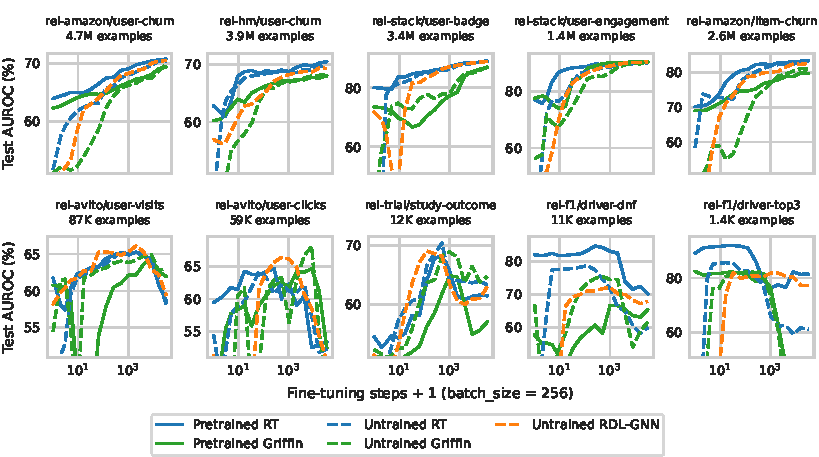
\includegraphics{auto-figures/learn-idv-auc.pdf}
\caption{Per-task test set learning curves on classification tasks for up to 32k fine-tuning steps (8M training examples, including
repetitions). X-axis is on log-scale.
}
\label{fig:learn-idv-auc}
\end{figure}

\begin{figure}[t]
\centering
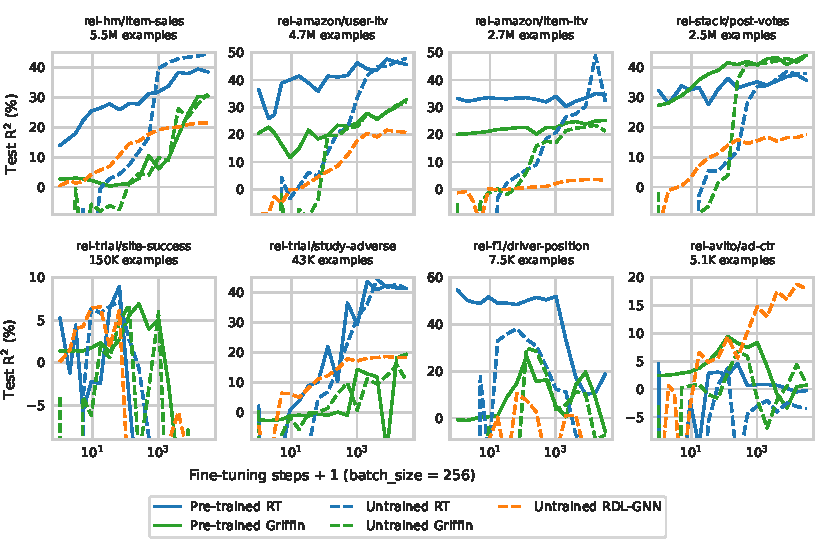
\includegraphics{auto-figures/learn-idv-r2.pdf}
\caption{
Per-task test set learning curves on regression tasks for up to 32k fine-tuning steps (8M training examples, including
repetitions). X-axis is on log-scale.
}
\label{fig:learn-idv-r2}
\end{figure}



\subsection{Supervised Learning in High-Resource Settings}
\label{appsec:ful-fine-tuning}

\paragraph{Setup.}
In Table~\ref{tab:fine-tuning},
we report results from full-dataset fine-tuning, using up to several million training examples and continuing until convergence (tens of thousands of steps).
We compare against schema-specific baselines (RDL-GNN, 
RelGNN, and 
RelGT), which cannot be pretrained, 
as well as schema-agnostic baselines (RelLLM and 
Griffin).
For RT and Griffin, we evaluate both untrained and pretrained initializations to assess the impact of pretraining. 
For all methods, the best checkpoint is selected based on validation set performance.
For RelGNN, RelGT, and RelLLM, we use the original training setups and hyperparameters. For Griffin, we increase the model size and update the sampling and pretraining procedures to be consistent with RT.

\begin{table}[t]
\CatchFileDef{\dataClf}{auto-tables/ft-auc.tex}{}
\CatchFileDef{\dataReg}{auto-tables/ft-r2.tex}{}
\centering
\scriptsize
\begin{tabular}{llrrrrrrrrr}
\toprule
\multirow{2}{*}{Dataset}
& \multirow{2}{*}{Task}
& \multirow{2}{*}{\makecell{Train\\set size\\(sorted)}}
& \multicolumn{3}{c}{Cannot be pretrained}
& \multicolumn{5}{c}{Can be pretrained} \\
\cmidrule(lr){4-6} \cmidrule(lr){7-11}
&
&
& \makecell{RDL\\GNN}
& \makecell{Rel\\GNN}
& \makecell{Rel\\GT}
& \makecell{Rel\\LLM}
& Griffin
& Griffin
& \makecell{RT\\(Ours)}
& \makecell{RT\\(Ours)} \\
\cmidrule{1-11}
\multicolumn{3}{r}{pretrained? $\rightarrow$}
& No
& No
& No
& Yes
& No
& Yes
& No
& Yes \\
\midrule
\multicolumn{11}{l}{
AUROC (\%) for $10$ binary classification tasks.
Higher is better.
Random/majority baseline is $50.0$.
} \\
\cmidrule{1-11}
\dataClf
\midrule
\multicolumn{11}{l}{
R$^2$ (\%) for $8$ regression tasks.
Higher is better.
Global-mean baseline is $0.0$.
} \\
\cmidrule{1-11}
\dataReg
\bottomrule
\end{tabular}
\caption{Supervised fine-tuning results. Models are trained on the full training set until convergence, with checkpoint selection based on validation performance. RT achieves the best mean AUROC and $R^2$ across tasks, surpassing both schema-specific (cannot be pretrained) and schema-agnostic (can be pretrained) baselines.
}
\label{tab:fine-tuning}
\end{table}

\paragraph{Observations.}
%1)
The pretrained RT achieves the best performance on average, achieving the highest mean AUROC and $R^2$.
On classification, it is outperformed on certain tasks by RelGNN, RelGT and RelLLM, but it is important to note that these methods utilize custom setups for each task, whereas RT uses a single unified hyperparameter setup across all experiments.
On regression, pretrained RT ranks best on average, substantially outperforming the second-best method across most tasks.
%2)
Overall, RT matches or exceeds the performance of schema-specific baselines while maintaining a general, schema-agnostic design, showing that generalization does not come at the expense of fine-tuning performance.
% %3) 
% Interestingly, the untrained RT outperfroms the pretrained variant on two regression tasks. % We should investigate this

\section{Context Window Ablations}
\label{app:cont_ablations}

\begin{table}[t]
\CatchFileDef{\dataClf}{auto-tables/ctx-auc.tex}{}
\CatchFileDef{\dataReg}{auto-tables/ctx-r2.tex}{}
\centering
\scriptsize
\begin{tabular}{llp{1em}rrrrp{1em}rrrr}
\toprule
Dataset $\downarrow$
& Task $\downarrow$
&
& \multicolumn{4}{c}{Zero-shot}
&
& \multicolumn{4}{c}{Fine-tuned} \\
\cmidrule{1-2} \cmidrule{4-7} \cmidrule{9-12}
\multicolumn{2}{r}{Ablated from context $\rightarrow$}
&
& none
& \makecell{col\\names}
& \makecell{self\\labels}
& \makecell{other\\labels}
&
& none
& \makecell{col\\names}
& \makecell{self\\labels}
& \makecell{other\\labels} \\
\midrule
\multicolumn{12}{l}{
AUROC (\%) for $10$ binary classification tasks.
Higher is better.
Random/majority baseline is $50.0$.
} \\
\cmidrule{1-12}
\dataClf
\midrule
\multicolumn{12}{l}{
R$^2$ (\%) for $8$ regression tasks.
Higher is better.
Global-mean baseline is $0.0$.
} \\
\cmidrule{1-12}
\dataReg
\bottomrule
\end{tabular}
\caption{
%\rr{}
Ablation study of context construction. To explain the zero-shot performance we remove column names, past labels from the target entity and labels from other entities.
To assess how much task-relevant information is lost, we repeat the same ablations in the fine-tuning setting.
Shading indicates the performance difference relative to the full context (none column).
% \mf{mmh. This figure here actually shows that there is not a lot to transfer besides the self-labels.}
}
\label{tab:context_ablations}
\end{table}

In Section~\ref{sec:context_ablation}, we introduced ablations of the context window to analyze the emergence of zero-shot performance. Here, we provide the full results of that study. Specifically, we systematically remove or perturb individual context components and report their effect on both zero-shot transfer and supervised fine-tuning performance.

\paragraph{Setup.}
In Table~\ref{tab:context_ablations}, we report results when shuffling column and table names, removing past labels from the target entity, or removing labels from other entities. For zero-shot evaluation, the ablations are applied directly to the sampled context used as input. For fine-tuning, models are trained to convergence with the same modified contexts. In addition, Table~\ref{tab:context_breakdown} provides statistics on the number of label cells (mean $\pm$ std. dev.) included in a context window of length $1024$ under our sampling procedure (Alg.~\ref{alg:sampler}).

\begin{table}[t]
\CatchFileDef{\dataClf}{manual-tables/ctx-stats-clf.tex}{}
\CatchFileDef{\dataReg}{manual-tables/ctx-stats-reg.tex}{}
\centering
\scriptsize
\begin{tabular}{llccc}
\toprule
Dataset
& Task
& \makecell{Target entity\\labels}
& \makecell{Other entity\\labels}
& \makecell{Unique\\labeled entities} \\
\midrule
\multicolumn{5}{c}{Binary Classification Tasks} \\
\cmidrule{1-5}
\dataClf
\cmidrule{1-5}
\multicolumn{5}{c}{Regression Tasks} \\
\cmidrule{1-5}
\dataReg
\bottomrule
\end{tabular}
\caption{
Breakdown of ``in-context labels'' sampled by Alg.~\ref{alg:sampler}.
Context length is $1024$ cells.
Numbers are (mean $\pm$ std. dev.; both rounded to the nearest integer).
\textbf{Target entity}, e.g., user, item, etc.,
is the one for which prediction is desired.
\textbf{Labels} refer to unmasked cells from the target column.
\textbf{Other entities} are reached via graph traversal.
Multiple labels are possible for the same entity
as the tasks are temporal.
%\rr{}
}
\label{tab:context_breakdown}
\end{table}

\paragraph{Observations.}
We find that zero-shot transfer primarily arises from the presence of past labels of the target entity. Removing these labels causes the largest drop in performance, whereas removing labels from other entities has a smaller effect. Shuffling column and table names also harms transfer, highlighting the importance of semantic signals from schema metadata. In the fine-tuning setting, classification performance is largely robust to these ablations, but regression tasks consistently benefit from access to past labels of the target entity.









\section{Architecture Ablations}
\label{app:ablations}

In Section~\ref{sec:layer_ablation}, we introduced ablations of the relational attention layers to assess their contribution to zero-shot transfer and fine-tuning performance. Here, we present the detailed results of that study. Specifically, we remove individual attention layers—column, feature, neighbor, or full/global—and analyze their effect across regression tasks, while classification results (showing minor differences) are provided in App.~\ref{app:ablations}.

Table~\ref{tab:attention_ablations_clf} shows the full Relational Attention layer ablations. We observe no clear patterns in the zero-shot setting, but during finetuning removing any layer results in a decrease in performance, except on the \emph{user-clicks} task, where the model is prone to overfit.

\begin{table}[t]
\CatchFileDef{\dataClf}{auto-tables/layer-auc.tex}{}
\CatchFileDef{\dataReg}{auto-tables/layer-r2.tex}{}
\centering
\scriptsize
\setlength{\tabcolsep}{4.5pt}
\begin{tabular}{llp{1em}rrrrrp{1em}rrrrrr}
\toprule
Dataset $\downarrow$
& Task $\downarrow$
&
& \multicolumn{5}{c}{Zero-shot}
&
& \multicolumn{5}{c}{Fine-tuned} \\
\cmidrule{1-2} \cmidrule{4-8} \cmidrule{10-14}
\multicolumn{2}{r}{Ablated attention $\rightarrow$}
&
& none
& col
& feat
& nbr
& full
&
& none
& col
& feat
& nbr
& full \\
\midrule
\multicolumn{14}{l}{
AUROC (\%) for $10$ binary classification tasks.
Higher is better.
Random/majority baseline is $50.0$.
} \\
\cmidrule{1-14}
\dataClf
\bottomrule
\end{tabular}
\caption{
Ablation studies on the attention layers of RT on classification tasks.
\textbf{col, feat, nbr, full} denote that
\textit{column-, feature-, neighbor-, full-} attention layers
are absent respectively.
Total parameter count is kept constant by increasing the number of layers.
Shading is proportional to difference from the \textbf{none} column.
}
\label{tab:attention_ablations_clf}
\end{table}














\begin{table}[t]
\CatchFileDef{\dataClf}{auto-tables/mask-auc.tex}{}
\CatchFileDef{\dataReg}{auto-tables/mask-r2.tex}{}
\centering
\scriptsize
\setlength{\tabcolsep}{4.5pt}
\begin{tabular}{llp{1em}rrrp{1em}rrrrr}
\toprule
Dataset $\downarrow$
& Task $\downarrow$
&
& \multicolumn{3}{c}{Zero-shot}
&
& \multicolumn{4}{c}{Fine-tuned} \\
\cmidrule{1-2} \cmidrule{4-6} \cmidrule{8-11}
\multicolumn{2}{r}{P(mask) $\rightarrow$}
&
& $0.0$
& $0.2$
& $0.4$
&
& $0.0$
& $0.2$
& $0.4$
& NP \\
\midrule
\multicolumn{11}{l}{
AUROC (\%) for $10$ binary classification tasks.
Higher is better.
Random/majority baseline is $50.0$.
} \\
\cmidrule{1-11}
\dataClf
\midrule
\multicolumn{11}{l}{
R$^2$ (\%) for $8$ regression tasks.
Higher is better.
Global-mean baseline is $0.0$.
} \\
\cmidrule{1-11}
\dataReg
\bottomrule
\end{tabular}
\caption{
Pretraining with multi-cell masking.
Masked cells contribute to the loss.
The target cell is always masked.
Other cells are masked with probability \textbf{P(mask)}.
\textbf{NP} denotes no pretraining.
Shading is proportional to difference from the P(mask) $=0.0$ column.
}
\end{table}


\subsection{\rev{Relational Attention Order Ablations}}
\label{app:order_ablations}

\begin{table}[t]
\CatchFileDef{\dataClf}{auto-tables/order-auc.tex}{}
\CatchFileDef{\dataReg}{auto-tables/order-r2.tex}{}
\centering
\scriptsize
\rev{
\begin{tabular}{llrrrrrrr}
\toprule
Dataset
& Task
& CFN
& CNF
& FCN
& FNC
& NCF
& NFC
& Parallel \\
\midrule
\multicolumn{9}{l}{
AUROC (\%) for $10$ binary classification tasks.
Higher is better.
Random/majority baseline is $50.0$.
} \\
\cmidrule{1-9}
\dataClf
\midrule
\multicolumn{9}{l}{
R$^2$ (\%) for $8$ regression tasks.
Higher is better.
Global-mean baseline is $0.0$.
} \\
\cmidrule{1-9}
\dataReg
\bottomrule
\end{tabular}
}
\caption{
\rev{
Different orders of relational attention layers.
\textbf{C, F, N} denote
\textit{column-, feature-, neighbor-} attention layers respectively.
The order of letters in the column headers
indicates the order of relational attention layers
applied sequentially.
\textbf{Parallel} denotes that
all three attention layers are applied in parallel
and their outputs are summed.
Results are shown for the zero-shot setting.
Experimental setup is same as followed in the main paper.
}
}
\label{tab:order_ablations}
\end{table}

Tab.~\ref{tab:order_ablations} shows the results of ablations on the order of relational attention layers. We observe no clear patterns, suggesting that the specific order of relational attention layers is not critical to performance.


% \clearpage   % or \newpage
\section{Baseline Implementations}
\label{app:baselines}


\subsection{Entity Mean}
\label{app:entity_mean}

The EntityMean baseline predicts the mean of past target-entity labels. When no past labels are available for the target entity, it falls back to the global mean of the target column on the training set. For computational efficiency, we report the metrics on a subsampled test set.


\subsection{LLM Prompt Construction}
\label{app:llm_prompting}

Large language models (LLMs) are evaluated under the same information regime as our relational
transformer (RT): input to both is constructed from the same context subgraph produced by our sampling algorithm (Alg.~\ref{alg:sampler}). In this graph, nodes correspond to database rows and edges represent
F$\to$P and P$\to$F links. We serialize the sampled entity graph into
\textbf{JSON}, which encodes relational structure.

\paragraph{Serialization procedure.}
We begin with the subgraph produced by the sampler. Serialization starts at the \emph{task node},
which specifies the prediction timestamp and links directly to the target entity for which the label
is to be predicted. From this target entity, we traverse the relational graph using both F$\to$P and
P$\to$F links. Each visited row is merged into the existing record in the case of F$\to$P link or further serialized and appended as a new entry to the list of linked entities in the case of
P$\to$F link.



\paragraph{Prompt components.}
Each prompt follows a fixed four-part structure: (i) a short dataset description; (ii) a description of the prediction task; (iii) the serialized graph context (a JSON of table–row objects) including the prediction timestamp \(t_0\); and (iv) a concise instruction specifying the expected output (“yes” or “no”). Dataset and task descriptions are adapted from prior work \citep{relbench}.

\paragraph{Full prompt example.}\mbox{}\par
\begin{lstlisting}[basicstyle=\ttfamily\scriptsize,
  breaklines=true,columns=fullflexible,keepspaces=true,showstringspaces=false]
You are a strict prediction assistant. Follow the instructions exactly.
# Database
Name: Stack Exchange
Description: Stack Exchange is a network of question-and-answer websites on different topics,
where questions, answers, and users are subject to a reputation award process. The reputation
system allows the sites to be self-moderating. The database includes detailed records of activity
including user biographies, posts and comments (with raw text), edit histories, voting, and
related posts. In our benchmark, we use the stats-exchange site.
# Task
Name: user-badge
Description: This task is to predict if this user will receive a new badge in the next 3 months or not.
# Input
- Database serialization starting from the target instance, expanding context by including rows
  reached via f2p (foreign to primary) and p2f (primary to foreign) relationships.
- The first timestamp in the sequence denotes the prediction time t0.
# Database serialization for the target entity
{
  "timestamp": "2021-01-01T00:00:00",
  "UserId": 211098,
  "Id": 211098,
  "AccountId": 12827220.0,
  "DisplayName": "Shashwat Tiwary",
  "Location": null,
  "ProfileImageUrl": null,
  "WebsiteUrl": null,
  "AboutMe": null,
  "CreationDate": "2019-09-15T05:33:35.413000",
  "add_badges": [
    {"Id": 383629, "UserId": 211098, "Class": 3, "Name": "Editor", "TagBased": false,
     "Date": "2019-09-15T07:40:23.563000"}
  ],
  "add_user-badge": [
    {"timestamp": "2020-10-01T00:00:00", "UserId": 211098, "WillGetBadge": "no"},
    {"timestamp": "2020-04-02T00:00:00", "UserId": 211098, "WillGetBadge": "no"},
    ...
    {"timestamp": "2019-10-03T00:00:00", "UserId": 211098, "WillGetBadge": "no"}
  ]
}
# Output
- Output exactly one word on a single line: yes or no.
- No units, no punctuation, no spaces, no commas, no extra text, no extra symbols, no new lines.
Make your prediction for the target entity at t0 using database serialization,
database description, and task description.
\end{lstlisting}
% \clearpage   % or \newpage



\paragraph{In-context labels.}
Due to the nature of our sampling algorithm, past (unmasked) labels from the target column can remain in the serialized JSON. For example, in the \texttt{user-badge} task (see full prompt above), the nested entries under \texttt{add\_user-badge} constitute such in-context labels. More details on the occurrence and distribution of these labels are provided in Table~\ref{tab:context_breakdown}.

% \paragraph{Evaluation.}
% For classification tasks we report AUROC, a threshold-free ranking metric. To obtain scores from
% LLM outputs, we take the probability assigned to the token ``yes'' as the model's prediction for
% positive class membership.




\subsection{Regression Results with LLM Baselines}
\label{app:llm_poor_regression}
In addition to classification, we evaluated zero-shot regression with LLMs of varying sizes under the same RT information regime. Across eight regression tasks, performance was consistently poor—smaller models even failed to produce stable numerical outputs  under strict prompting. We attribute this to unconstrained number generation and a context not optimized for LLM regression. Prior work shows that carefully selecting and formatting in-context examples can substantially improve results \citep{nafar2025learning}. Given these limitations, we do not report detailed regression metrics.

\subsection{Griffin}
To ensure a fair comparison with Griffin, we scale its hidden dimension from 512 to 728, resulting in a comparable parameter count to RT (22.8M vs.\ 22.3M). We also match the training setup by adopting both the leave-one-database-out and continued pre-training regimes. However, since the Griffin implementation does not support joint training on forecasting and autocomplete tasks, we restrict it to forecasting tasks only.

\begin{table}[t]
\CatchFileDef{\data}{auto-tables/zs-r2.tex}{}
\centering
\scriptsize
\begin{tabular}{llrrrrrrrrr}
\toprule
\multicolumn{2}{r}{Target DB $\in$ pretraining? $\rightarrow$}
& \multicolumn{3}{c}{Maybe}
& \multicolumn{3}{c}{No}
& \multicolumn{3}{c}{Yes}
\\
\cmidrule(lr){3-5} \cmidrule(lr){6-8} \cmidrule(lr){9-11}
Dataset $\downarrow$
& Task $\downarrow$
& Gemma
& Gemma
& Gemma
& \makecell{Entity\\Mean}
& Griffin
& \makecell{RT\\(ours)}
& \makecell{Rel\\LLM}
& Griffin
& \makecell{RT\\(ours)}\\
\cmidrule{1-11}
\multicolumn{2}{r}{Parameter count $\rightarrow$}
& 4B
& 12B
& 27B
& 0
& 22M
& 22M
& 3B
& 22M
& 22M \\
\midrule
\data
\bottomrule
\end{tabular}
\caption{
Zero-shot R$^2$ (\%) for $8$ regression tasks.
Higher is better.
Global mean baseline is $0.0$.
Setup is same as Table~\ref{tab:zero-shot-clf}.
}
\label{tab:zero-shot-reg}
\end{table}

\section{Relational Transformer Block}

Algorithm~\ref{alg:transformer_block} illustrates the architecture of a single Relational Transformer Block. This block consists of a series of attention mechanisms: a column attention layer, a feature attention layer, a neighbor attention layer, and a global attention layer, each with its own specific relational inductive bias. These Relational Attention layers are followed by a feed-forward network (MLP) for further processing.
\begin{algorithm}[ht]
\DontPrintSemicolon
\KwIn{input token representations $\X \in \mathbb{R}^{n \times d}$}
\KwOut{output token representations $\X \in \mathbb{R}^{n \times d}$}
$\X \gets \X + \textsc{Norm}(\;\textsc{MHA}(\X; \M^\text{column})\;)$\;
$\X \gets \X + \textsc{Norm}(\;\textsc{MHA}(\X; \M^\text{feature})\;)$\;
$\X \gets \X + \textsc{Norm}(\;\textsc{MHA}(\X; \M^\text{neighbor})\;)$\;
$\X \gets \X + \textsc{Norm}(\;\textsc{MHA}(\X; \M^\text{full})\;)$\;
$\X \gets \X + \textsc{Norm}(\;\textsc{MLP}(\X)\;)$\;
\KwRet{$\X$}\;
\caption{
A transformer block in RT.
}
\label{alg:transformer_block}
\end{algorithm}
